\documentclass[border=4pt]{standalone}
\usepackage{amsmath,amssymb}
\usepackage{tikz}
\begin{document}
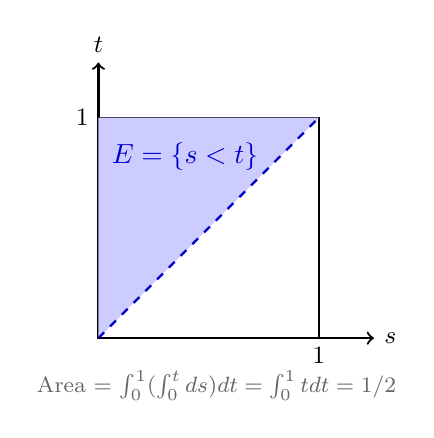
\begin{tikzpicture}[font=\small]
  \draw[->, thick] (0,0) -- (3.5,0) node[right] {$s$};
  \draw[->, thick] (0,0) -- (0,3.5) node[above] {$t$};

  \draw[thick] (0,0) rectangle (2.8, 2.8);
  \node[below] at (2.8,0) {$1$};
  \node[left] at (0,2.8) {$1$};

  % Triangle E = {s < t}
  \fill[blue!20] (0,0) -- (0,2.8) -- (2.8,2.8) -- cycle;
  \draw[thick, dashed, blue!80!black] (0,0) -- (2.8,2.8);
  \node[blue!80!black, font=\bfseries] at (1.1, 2.3) {$E = \{s < t\}$};

  \node[font=\footnotesize, text=gray!80!black] at (1.5, -0.6) 
    {Area = $\int_0^1 (\int_0^t ds) dt = \int_0^1 t dt = 1/2$};
\end{tikzpicture}
\end{document}
